\chapter{Classificazione}
\label{chapter:classification}

Il cuore del progetto riguarda la classificazione delle attività mediante i dati ottenuti. 

Ho optato per l'utilizzo di Keras \cite{keras}.
Si tratta di una libreria open-source per le reti neurali che astrae lo sviluppo rendendolo più comprensibile, 
pur mantenendo pieno supporto alle librerie di più basso livello (es. Tensorflow \cite{tensorflow}) su cui si basa.


\section{Caricamento dei dati}
Il passaggio che precede l'apprendimento è il recupero dei dati collezionati nei file CSV.

\begin{figure}[H]
    \centering
    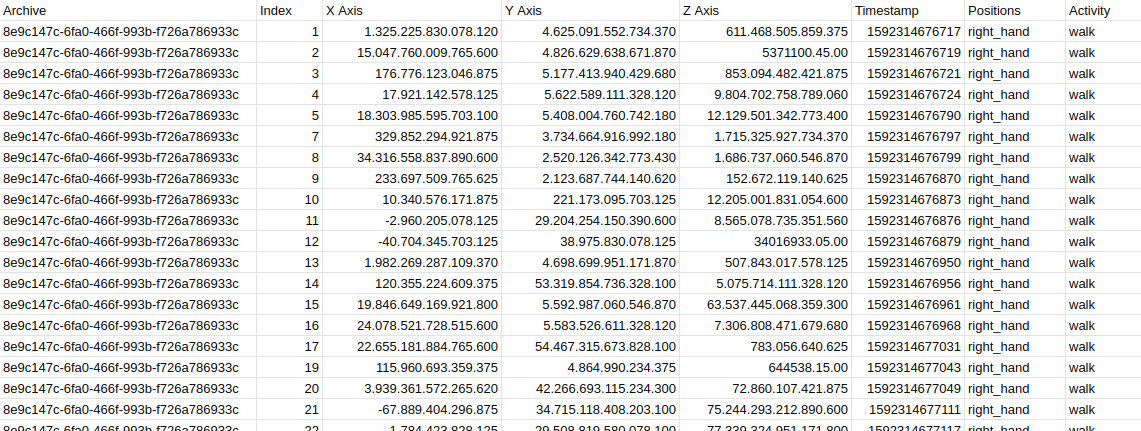
\includegraphics[scale = 0.40]{assets/images/examples/dataset-data-example.png}
    \caption{Esempio di dati contenuti nel file CSV}
\end{figure}

Dopo la sola lettura è già possibile ottenere una chiara visualizzazione grafica della suddivisione per attività dei dati presenti.

\begin{figure}[H]
    \centering
    \includegraphics[scale = 0.40]{assets/images/activity-type-graph_acc.png}
    \centering
    \includegraphics[scale = 0.40]{assets/images/activity-type-graph-gyro.png}
    \caption{Visualizzazione della suddivisione dei dati per i due sensori}
\end{figure}


\newpage
I dataset sono relativi ai sensori attivi sull'applicazione, ovvero accelerometro e giroscopio.
Entrambi contengono la stessa tipologia di informazioni (i valori dei tre assi, il timestamp e il posizionamento del dispositivo). 
Nelle procedure seguenti considererò quindi il singolo dataset, ricordando però di dover applicare i passaggi indistintamente ad entrambi.

\section{Apprendimento e Test}

L'intera mole di dati necessita un partizionamento per differenziare i dati che saranno utilizzati per 
l'\textit{apprendimento} e quelli che saranno utilizzati per il \textit{test}.

Personalmente ho scelto una semplice suddivisione che prevede l'utilizzo di $\frac{4}{5}$ dei dati per il \textit{train} e 
la parte restante ($\frac{1}{5}$) per il \textit{test}.

È indispensabile non sovrapporre queste frazioni se non si vuole ottenere una valutazione dell'efficienza falsata.

\subsection{Preparazione dei dati}
Ci si aspetta che, fornita una serie di caratteristiche (i tre assi x, y, z, il valore temporale e 
la posizione del dispositivo), la rete neurale dia in risposta un'etichetta rappresentate l'attività associata.

Dobbiamo quindi organizzare i dati in nostro possesso in modo da renderlo possibile.

\subsubsection{Trasformazione del valore temporale}
Tra le caratteristiche abbiamo i \textit{timestamp}s che però rappresentano il tempo assoluto, 
ovvero il momento esatto di svolgimento dell'attività durante la raccolta dei dati.

Il momento esatto non è in alcun modo rilevante nella classificazione, ma a partire da questo è possibile ricavare il tempo trascorso 
tra l'acquisizione di una tripla di dati (x, y, z) e l'acquisizione di quella immediatamente successiva.
Posso presumere una somiglianza in tali distanze temporali durante lo svolgimento di una uguale attività.

\subsubsection{Normalizzazione dei dati}
La rete neurale accetta in ingresso valori compresi tra 0 e 1. Eseguo una semplice normalizzazione sui dati delle caratteristiche.
\begin{listing}[H] 
    \inputminted[frame=single,framesep=10pt]{python}{snippets/normalize_data.py}
    \caption{Banale normalizzazione dei dati}
\end{listing}

\subsubsection{Creazione dei segmenti e delle etichette}
La parte principale dell'intero adattamento risulta essere quella che suddivide i dati in un formato che possa 
realizzare l'associazione tra una serie di caratteristiche e una etichetta.

Per realizzare ciò i record sono presi a gruppi, anche sovrapposti (così come si vede in figura \ref{fig:create_segments_and_labels}). 
Ogni raggruppamento sarà caratterizzato da 
\begin{itemize}
    \item un segmento contenente i record con le sole caratteristiche
    \item l'etichetta più frequente
\end{itemize}

\begin{figure}[H]
  \centering
  \includesvg[scale = 0.6]{assets/graphs/create_segments_and_labels.svg}
  \caption{Creazione dei segmenti e delle etichette}
  \label{fig:create_segments_and_labels}
\end{figure}

\begin{figure}[H]
  \centering
  \includesvg[scale = 0.6]{assets/graphs/segments_and_labels.svg}
  \caption{Risultato dopo la creazione dei segmenti e delle etichette}
  \label{fig:segments_and_labels}
\end{figure}

Alla fine del processo ho quindi ottenuto una serie di segmenti di dati a cui posso singolarmente associare una determinata
etichetta identificativa.

\newpage
\subsection{Creazione della rete neurale}
Una volta generati i dati nel formato supportato da \textit{Keras} procedo alla creazione di 
una rete neurale che abbia
\begin{itemize}
    \item in input il formato dei dati appena generato
    \item 5 strati di 100 nodi connessi
    \item in output il calcolo di propabilità per ogni classe
\end{itemize}
\begin{listing}[H] 
    \inputminted[frame=single,framesep=10pt]{python}{snippets/dnn_create.py}
    \caption{Creazione della DNN}
\end{listing}
Per poi procedere all'apprendimento.
\begin{listing}[H] 
    \inputminted[frame=single,framesep=10pt]{python}{snippets/dnn_fit.py}
    \caption{Apprendimento della rete neurale}
\end{listing}

\begin{figure}[H]
    \centering
    \includegraphics[scale = 0.45]{assets/images/modal_accuracy_data_loss_acc.png}
    \centering
    \includegraphics[scale = 0.45]{assets/images/modal_accuracy_data_loss_gyro.png}
    \caption{Statistiche del modello ottenuto}
\end{figure}

\subsection{Testing della rete neurale}
Il test della rete neurale creata avviene mediante l'uso dei dati che avevamo precedentemente separato dal dataset iniziale.

L'intento è quello di effettuare una predizione con i dati di test, di cui però si conoscono già i risultati. 
Sarà quindi immediato trovare l'efficienza del modello creato mediante un banale confronto tra i dati ipotizzati 
dalla rete neurale e i risultati corretti.

La qualità dei dati può essere visualizzata mediante una \textit{matrice di confusione} che fornisce una rappresentazione grafica del confronto appena descritto.

\begin{figure}[H]
    \centering
    \includegraphics[scale = 0.45]{assets/images/confusion_matrix_acc.png}
    \centering
    \includegraphics[scale = 0.45]{assets/images/confusion_matrix_gyro.png}
    \caption{Statistiche del modello ottenuto}
\end{figure}

\section{Predizioni}
In maniera del tutto equivalente a quanto già visto durante l'apprendimento, per effettuare una predizione sfruttando
la rete neurale allenata forniremo in input una serie di segmenti e attenderemo che il classificatore ci fornisca in risposta
una serie di etichette ipotizzate.

